\documentclass[9pt, aspectratio=169]{beamer}

\usetheme{metropolis}
\setbeamertemplate{itemize items}{\faAngleRight}

\metroset{titleformat=smallcaps,block=fill,numbering=counter,progressbar=frametitle,sectionpage=none}
\setbeamersize{text margin left=5mm,text margin right=5mm} 
% \input{embed_video}
\usepackage{fontspec,minted}
\usepackage[scale=1]{ccicons}
\usepackage{metalogo}
\usepackage{xcolor,colortbl}
\usepackage{multicol,multirow,booktabs}
\usepackage{appendixnumberbeamer}
\usepackage{graphicx}
\usepackage{mismath}
\usepackage{bm}
\usepackage{fontawesome5}
\usepackage{csquotes}
\usepackage[backend=biber, natbib, sorting=nyt, doi=true, url=false, url=false, isbn=false, maxbibnames=10]{biblatex}
\addbibresource{../utils/refs.bib}

\usepackage[spanish, es-nodecimaldot]{babel}
\deftranslation[to=spanish]{Definition}{Definición}
\deftranslation[to=spanish]{Theorem}{Teorema}
\deftranslation[to=spanish]{Example}{Ejemplo}

\usepackage{mathtools, mathrsfs}
\usefonttheme{professionalfonts}
\usepackage{textcomp, wasysym}

\setsansfont[BoldFont={Iwona Heavy}, Numbers={Lining, Proportional}]{Iwona Light}
\setmonofont[Scale=MatchLowercase]{Hack Nerd Font Mono}

\setbeamercolor{alerted text}{fg=red,bg=black!2}
\setbeamercolor{progress bar}{fg=red,bg=red!2}
\setbeamertemplate{itemize item}{\faCaretRight}
\setbeamertemplate{itemize subitem}{ \faAngleRight}
\setbeamertemplate{blocks}[shadow=false]
\setbeamercolor{block title}{bg=black!30,fg=red}
\setbeamercolor{block body}{bg=black!20,fg=black}
\setbeamertemplate{theorem begin}
{%
\begin{\inserttheoremblockenv}
{%
\inserttheoremheadfont
%{Teorema:}
\inserttheoremname
\ifx\inserttheoremaddition\@empty\else\ : \inserttheoremaddition\fi%
\inserttheorempunctuation
}%
}
\setbeamertemplate{theorem end}{\end{\inserttheoremblockenv}}
\makeatother


 
\usepackage{gensymb,amssymb}
\usepackage{siunitx}
\DeclareSIUnit{\nada}{\relax}
\usepackage{upquote}
\usepackage{cancel}
\usepackage{algpseudocode}
\algrenewcommand\algorithmicrequire{\textbf{Requiere}}
\algrenewcommand\algorithmicensure{\textbf{Devuelve}}
\setbeamertemplate{blocks}[shadow=false]

\newcommand{\cx}{\column{0.5\textwidth}}
\newcommand{\cw}[1]{\column{#1\textwidth}}

\author{Manuel Carlevaro}
\date{{\tiny Departamento de Ingeniería Mecánica \\
             Grupo de Materiales Granulares - UTN FRLP \\
             manuel.carlevaro@gmail.com }}
\institute{
  \vspace{6em}
  \centering
  {\tiny
  Cálculo Avanzado \enspace • \enspace 2025 \\
    \faLinux \- $\cdot$ \- \fontspec{TeX Gyre Pagella}\XeLaTeX \- $\cdot$ \- \ccbysa }
}

%% Operadores
\DeclareMathOperator{\sen}{sen}
\DeclareMathOperator{\senc}{senc}
\DeclareMathOperator{\sign}{sign}
\DeclareMathOperator{\Tr}{Tr}
\DeclareMathOperator{\rg}{rg}
\DeclareMathOperator{\cond}{cond}
\newcommand{\T}[1]{\underline{\bm{#1}}}
\newcommand{\uvec}[1]{\hat{\bm{#1}}}

\usepackage{hyperref}
\hypersetup{
    colorlinks,
    citecolor=blue,
    filecolor=black,
    linkcolor=blue,
    urlcolor=blue
}
\urlstyle{same}

%% Códigos
\usepackage{minted}
\newminted[cpp]{cpp}{linenos,fontsize=\footnotesize,frame=lines,numbersep=4pt}
\newmintedfile[cppcode]{cpp}{linenos,fontsize=\footnotesize,frame=lines,numbersep=4pt}
\newcommand{\mic}[1]{\mintinline{C++}{#1}}

\newminted[py]{python}{linenos,fontsize=\footnotesize,frame=lines,numbersep=4pt}
\newminted[pyc]{pycon}{linenos,fontsize=\footnotesize,frame=lines,numbersep=4pt} % Consola de Python
\newminted[ipy3]{ipython3}{linenos,fontsize=\footnotesize,frame=lines,numbersep=4pt} % Consola de iPython3
\newmintedfile[pycode]{python}{linenos,fontsize=\footnotesize,frame=lines,numbersep=4pt}

\newmintedfile[makef]{basemake}{linenos,fontsize=\footnotesize,frame=lines,numbersep=4pt}
\definecolor{bg}{RGB}{22,43,58}
\newminted[shell]{console}{linenos=false,fontsize=\footnotesize,breaklines=true, frame=single} % Linea de comandos
\renewcommand\listingscaption{Código}

\makeatletter
\AtBeginEnvironment{minted}{\dontdofcolorbox}
\def\dontdofcolorbox{\renewcommand\fcolorbox[4][]{##4}}
\makeatother

% uso:
% Ejemplo de uso explícito:
% \begin{py}
% >>> list("abcd")
% ['a', 'b', 'c', 'd']
% \end{py}
% 
% Ahora ejemplo de código en file:
% \pycode{Chapters/intro/code/hola.py}
% 
% También se puede poner un sector del file:
% \pycode[firstline=6, lastline=7]{Chapters/intro/code/hola.py}
% 
% También se puede poner código \textit{inline}: \mip{print('¡Hola mundo!')} y en una sola línea:
% \slp|if __name__ == '__main__')|
% 
% Por último, se puede poner el código en un entorno \textit{float}, esto es, como las tablas y las figuras, con un caption y un label para luego hacer referencias, como por ejemplo al Código \ref{code:hola}.


\usepackage{tikz}
\usetikzlibrary{shapes,shadows,arrows,positioning,matrix,chains,backgrounds,fit}

\tikzset{
    %Define standard arrow tip
    >=stealth',
    %Define style for boxes
    obj/.style={
           rectangle,
           rounded corners,
           draw, very thick,
           text width=10em, fill=green!20,
           minimum height=2em,
           text centered, drop shadow},
    proc/.style={
	    rectangle, rounded corners,
	    draw,fill=red!50,very thick,
	    text width=8em,minimum height=2em,
	    text centered, drop shadow},
    % Define arrow style
    pil/.style={
           ->,
           thick,
           shorten <=2pt,
           shorten >=2pt,}
}

\setbeamertemplate{bibliography item}{%
  \ifboolexpr{ test {\ifentrytype{book}} or test {\ifentrytype{mvbook}}
    or test {\ifentrytype{collection}} or test {\ifentrytype{mvcollection}}
    or test {\ifentrytype{reference}} or test {\ifentrytype{mvreference}} }
    {\setbeamertemplate{bibliography item}{\faBook}}
    {\ifentrytype{online}
            {\setbeamertemplate{bibliography item}{\faGlobe}}
   {\setbeamertemplate{bibliography item}{\faFileText}}}%
  \usebeamertemplate{bibliography item}}

\defbibenvironment{bibliography}
  {\list{}
     {\settowidth{\labelwidth}{\usebeamertemplate{bibliography item}}%
      \setlength{\leftmargin}{\labelwidth}%
      \setlength{\labelsep}{\biblabelsep}%
      \addtolength{\leftmargin}{\labelsep}%
      \setlength{\itemsep}{\bibitemsep}%
      \setlength{\parsep}{\bibparsep}}}
  {\endlist}
  {\item}
\newcommand{\bcite}[1]{\citeauthor{#1}, \citetitle{#1} (\citeyear{#1})}


\title{Transformada de Laplace}
\subtitle{Transformada de Laplace. Transformada inversa. Solución de problemas con condiciones iniciales.}

\DeclareMathOperator{\TL}{\mathscr{L}}

\begin{document}
\maketitle

\begin{frame}{Transformada de Laplace}
	\begin{columns}[c]
		\cw{0.4}
		\textbf{Motivación:}
		\begin{center}
			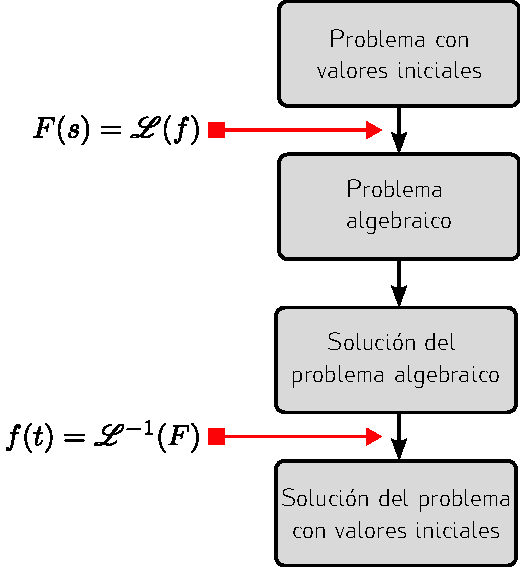
\includegraphics[ height=0.75\textheight ]{figs/fig-01.pdf}
		\end{center} \pause

		\cw{0.6}
		\begin{definition} [Transformada de Laplace]
			Sea $f(t)$ definida para todo $t \geq 0$. Su transformada de Laplace se define:
			\[ F(s) = \mathscr{L}(f) = \int_0^{\infty} e^{-s t} f(t) \, dt \]
		\end{definition} \pause

		\begin{theorem}[Existencia]
			Si $f(t)$ está definida y es continua a tramos en cada intervalo finito de $\mathbb{R^+}$, y satisface la condición
			\[ |f(t)| \leq M e^{k t} \text{ (restricción de crecimiento exponencial) } \]
			para algunas constantes, $M$ y $k$, entonces existe $\mathscr{L}(f), \; \forall s > k$.
		\end{theorem} \pause
		Si $F(s) = \mathscr{L}[f(t)]$, $f(t)$ es la \textbf{transformada inversa} de $F(s)$:
		\[ f(t) = \mathscr{L}^{-1} [F(s)] \]

		Por lo tanto: $\mathscr{L}^{-1}[\mathscr{L}(f)] = f$ y $\mathscr{L}[\mathscr{L}^{-1}(F)] = F$.
	\end{columns}
\end{frame}

\begin{frame}{Transformada integral}
	\textbf{Caso general:}
	\[ (Tf)(u) = \int_{t_1}^{t_2} f(t) \, K(t, u) \, dt \\ = F(u) \]
	donde $K(t, u)$ es la función \textbf{núcleo} o \textbf{kernel}.

	Cuando $K$ tiene asociado un \textit{kernel inverso} $K^{-1}(u, t)$, se puede definir (más o menos) la transformación inversa:
	\[ f(t) = \int_{u_1}^{u_2} (Tf)(u) \, K^{-1}(u, t) \, dt \]

	Si el kernel es \textbf{simétrico}: $K(t, u) = K(u, t) \mapsto$ operadores auto-adjuntos.

\end{frame}

\begin{frame}{Caso general: ejemplos}

	\begin{center}
		\begin{tabular}{llcccc}
			\toprule
			\textbf{Transformada} & \textbf{Símbolo} & $K$                             & $(t_1, t_2)$        & $K^{-1}$                        & $(u_1, u_2)$             \\
			\midrule
			Fourier               & $\mathscr{F}$    & $\frac{e^{-iut}}{\sqrt{2 \pi}}$ & $(-\infty, \infty)$ & $\frac{e^{+iut}}{\sqrt{2 \pi}}$ & $(-\infty, \infty)$      \\
			Fourier seno          & $\mathscr{F}_s$  & $\sqrt{\frac{2}{\pi}} \sen(ut)$ & $(0, \infty)$       & $\sqrt{\frac{2}{\pi}} \sen(ut)$ & $(0, \infty)$            \\
			Fourier coseno        & $\mathscr{F}_c$  & $\sqrt{\frac{2}{\pi}} \cos(ut)$ & $(0, \infty)$       & $\sqrt{\frac{2}{\pi}} \cos(ut)$ & $(0, \infty)$            \\
			Laplace               & $\mathscr{L}$    & $e^{-ut}$                       & $(0, \infty)$       & $\frac{e^{+ut}}{2 \pi i}$       & $(c-i\infty, c+i\infty)$ \\
			Laplace bilateral     & $\mathscr{B}$    & $e^{-ut}$                       & $(-\infty, \infty)$ & $\frac{e^{+ut}}{2 \pi i}$       & $(c-i\infty, c+i\infty)$ \\
			Hilbert               & $\mathcal{H}il$  & $\frac{1}{\pi} \frac{1}{u-t}$   & $(-\infty, \infty)$ & $\frac{1}{\pi} \frac{1}{u-t}$   & $(-\infty, \infty)$      \\
			Legendre              & $\mathcal{J}$    & $P_n(t)$                        & $(-1, 1)$           & (*)                             & $(0, \infty)$            \\
			\bottomrule
		\end{tabular}
	\end{center}
	\begin{align*}
		\text{(*) }\mathcal{J}[f(x)] = \tilde{f}(n) & = \int_{-1}^{1} P_n(x) \, f(x) \, dx                                 \\
		\mathcal{J}^{-1}[\tilde{f}(n)]              & = f(t) = \sum_{n = 0}^{\infty} \frac{2 n + 1}{2} \tilde{f}(n) P_n(x)
	\end{align*}
\end{frame}

\begin{frame}{Ejemplos}
	\begin{columns}[t]
		\cx
		$f(t) = 1, \, t \geq 0$
		\begin{align*}
			\mathscr{L}(f) = \mathscr{L}(1) & = \int_0^{\infty} e^{-st} \, dt                                                      \\
			                                & = \lim_{T \rightarrow \infty} \int_0^T 1 \cdot e^{-s t} \, dt                        \\
			                                & = \lim_{T \rightarrow \infty} \left[ -\frac{1}{s} e^{-s t} \right]_0^T               \\
			                                & = \lim_{T \rightarrow \infty} \left[ -\frac{1}{s} e^{-s T} + \frac{1}{s} e^0 \right] \\
			                                & = \frac{1}{s}
		\end{align*}
		\[ \boxed{ \mathscr{L}(1) = \frac{1}{s} } \]
		\pause

		\cx
		$f(t) = e^{at}, \, t \geq 0$
		\begin{align*}
			\mathscr{L} (e^{at}) & = \int_0^{\infty} e^{-st} \, e^{at} \, dt               \\
			                     & = \left. \frac{1}{a - s} e^{-(s-a)t} \right|_0^{\infty} \\
			                     & = \frac{1}{s -a}
		\end{align*}
		\[ \boxed{ \mathscr{L}(e^{at}) = \frac{1}{s -a}} \]
		cuando $s -a > 0$.
	\end{columns}
\end{frame}

\begin{frame}{Linealidad}
	\begin{columns}[t]
		\cx
		\begin{theorem}[Linealidad de $\mathscr{L}$]
			Para funciones $f(t)$ y $g(t)$ cuyas transformadas de Laplace existan, y para dos constantes arbitrarias $a$ y $b$, se cumple que:
			\[ \mathscr{L}[a f(t) + b g(t)] = a \mathscr{L}[f(t)] + b \mathscr{L}[g(t)] \]
		\end{theorem} \pause

		\textbf{Ejemplo:}
		Hallar las transformadas de $\cosh at$ y $\senh at$.

		Dado que:
		\begin{align*}
			\cosh at & = \frac{1}{2} (e^{at} + e^{-at}) \\
			\senh at & = \frac{1}{2} (e^{at} - e^{-at}) \\
		\end{align*}

		\cx
		Por la linealidad:
		\begin{align*}
			\mathscr{L}(\cosh at) & = \frac{1}{2} [\mathscr{L}(e^{at}) + \mathscr{L}(e^{-at})]     \\
			                      & = \frac{1}{2} \left( \frac{1}{s - a} + \frac{1}{s + a} \right) \\
			                      & = \frac{s}{s^2 - a^2}
		\end{align*}

		\begin{align*}
			\mathscr{L}(\senh at) & = \frac{1}{2} [\mathscr{L}(e^{at}) - \mathscr{L}(e^{-at})]     \\
			                      & = \frac{1}{2} \left( \frac{1}{s - a} - \frac{1}{s + a} \right) \\
			                      & = \frac{a}{s^2 - a^2}
		\end{align*}
	\end{columns}
\end{frame}

\begin{frame}{Transformada de la derivada}
	\begin{theorem}[Transformada de $f'$]
		Sea $f$ continua en $[0, \infty)$, con $f'$ continua a tramos en $[0, k]$ para todo $k > 0$, y $\lim_{k \rightarrow \infty} e^{-s k} f(k) = 0$ si $s > 0$. Entonces:
		\[ \mathscr{L}[f'(t)] = s F(s) - f(0) \]
	\end{theorem}

	{ \small
	\begin{proof}
		\vspace{1em}
		\begin{columns}[t]
			\cw{0.45}
			De la definición, integrando por partes:
			\begin{align*}
				\int_0^k e^{-st} f'(t) \, dt & = \left[ e^{-st} f(t) \right]_0^k - \int_0^k -s e^{-st} f(t) \, dt \\
				                             & = e^{-sk}f(k) - f(0) + s \int_0^k e^{-st} f(t) \, dt
			\end{align*}

			\cw{0.45}
			Tomando el límite $k \rightarrow \infty$:
			\begin{align*}
				\mathscr{L}[f'(t)] & = \lim_{k \rightarrow \infty} \left[ e^{-sk} f(k) - f(0) + s \int_0^k e^{-st} f(t) \, dt \right] \\
				                   & = -f(0) + s \int_0^{\infty} e^{-st} f(t) \, dt = -f(0) + s F(s)
			\end{align*}
		\end{columns}
	\end{proof}
	}
\end{frame}

\begin{frame}{Transformada de derivadas superiores}
	\begin{columns}[t]
		\cx
		Si $f$ y $f'$ son continuas para $t \geq 0$, cumplen la restricción de crecimiento exponencial y $f''$ es continua por tramos en cada intervalo finito en $\mathbb{R}^{+}$:
		\[ \mathscr{L}(f'') = s^2 \mathscr{L}(f) - s f(0) - f'(0) \]

		Aplicamos el teorema anterior a $f''$:
		\begin{align*}
			\mathscr{L}(f'') & = s \mathscr{L}(f') - f'(0)           \\
			                 & = s [s \mathscr{L}(f) - f(0)] - f'(0) \\
			                 & = s^2 \mathscr{L}(s) - s f(0) - f'(0)
		\end{align*}
		\pause

		\cx
		Transformada de derivada $n-$ésima:

		Si $f$, $f', \cdots, f^{(n-1)}$ son continuas para todo $t \geq 0$ y satisfacen la restricción de crecimiento exponencial, y si $f^{(n)}$ es una función continua por tramos en cada intervalo finito en $\mathbb{R}^+$, entonces la transformada de $f^{(n)}$ satisface:

		\begin{multline*}
			\mathscr{L}[f^{(n)}] = s^n \mathscr{L}(f) - s^{n-1} f(0) \\
			- s^{n-2} f'(0) - \cdots f^{(n-1)}(0)
		\end{multline*}
	\end{columns}
\end{frame}

\begin{frame}{Ejemplos}
	\begin{columns}[t]
		\cx
		\textbf{Transformada de $\cos \omega t$:}

		$f(t) = \cos \omega t$, $f(0) = 1, \, f'(0) = 0, \, f''(t) = -\omega^2 \cos \omega t$:

		\[ \mathscr{L}(f'') = s^2 \mathscr{L}(f) - s = -\omega^2 \mathscr{L}(f) \]

		\[ \boxed{ \mathscr{L}(\cos \omega t) = \frac{s}{s^2 + \omega^2} } \]
		\pause

		\cx
		\textbf{Transformada de $\sen \omega t$:}

		$g(t) = \sen \omega t$, $g(0) = 0, \, g'(t) = \omega \cos \omega t$:

		\[ \mathscr{L}(g') = s \mathscr{L}(g) = \omega \mathscr{L}(\cos \omega t) \]

		\[ \boxed{\mathscr{L}(\sen \omega t) =  \frac{\omega}{s^2 + \omega^2} } \]
	\end{columns}
\end{frame}

\begin{frame}{Tabla de transformadas más comunes}
\begin{center}
\begin{tabular}{cccccc}
  \toprule
\( f(t) \) & \( \mathcal{L}\{f(t)\} \) & \( f(t) \) & \( \mathcal{L}\{f(t)\} \) & \( f(t) \) & \( \mathcal{L}\{f(t)\} \) \\
\midrule
\( 1 \) & \( \frac{1}{s} \) & \( \cos(at) \) & \( \frac{s}{s^2 + a^2} \) & \( \delta(t) \) & \( 1 \) \\
\( t \) & \( \frac{1}{s^2} \) & \( \sin(at) \) & \( \frac{a}{s^2 + a^2} \) & \( \delta(t - a) \) & \( e^{-as} \) \\
\( t^n \) & \( \frac{n!}{s^{n+1}} \) & \( \sinh(at) \) & \( \frac{a}{s^2 - a^2} \) & \( u(t - a) \) & \( \frac{e^{-as}}{s} \) \\
\( e^{at} \) & \( \frac{1}{s - a} \) & \( \cosh(at) \) & \( \frac{s}{s^2 - a^2} \) & \( e^{-at}f(t) \) & \( F(s + a) \) \\
\( e^{at}t \) & \( \frac{1}{(s - a)^2} \) & \( t e^{at} \) & \( \frac{1}{(s - a)^2} \) & \( f'(t) \) & \( sF(s) - f(0) \) \\
\( \frac{\sin(at)}{t} \) & \( \tan^{-1}\left( \frac{a}{s} \right) \) & \( \frac{1 - e^{-at}}{t} \) & \( \ln\left( \frac{s + a}{s} \right) \) & \( f''(t) \) & \( s^2 F(s) - sf(0) - f'(0) \) \\
\( \int_0^t f(\tau)\, d\tau \) & \( \frac{F(s)}{s} \) & \( \frac{1}{\sqrt{t}} \) & \( \sqrt{\frac{\pi}{s}} \) & \( \frac{J_0(at)}{t} \) & \( \frac{1}{\sqrt{s^2 + a^2}} \) \\
\bottomrule
\end{tabular}
\end{center}
\end{frame}

\begin{frame}{Ecuaciones diferenciales: problema con valores iniciales}
	\begin{columns}[t]
		\cx
		$f'' + a f' + b f = r(t), \; f(0) = K_0, \; f'(0) = K_1$ \pause

		\begin{itemize}
			\item \textbf{Paso 1:}  $t \mapsto s$
			      \[ [s^2 F - s f(0) - f'(0)] + a[s F - f(0)] + b F = R(s) \]
			      \[ (s^2 + a s + b) F = (s + a) f(0) + f'(0) + R(s) \]
			      \pause

			\item \textbf{Paso 2:} Resolver $F(s)$

			      \textbf{Función transferencia:}
			      \[ Q(s) = \frac{1}{s^2 + a s + b} = \frac{1}{\left(s + \dfrac{1}{2} a \right)^2 + b - \dfrac{1}{4} a^2} \]
			      \[ F(s) = [(s + a) f(0) + f'(0)] Q(s) + R(s) Q(s) \]
		\end{itemize}
		\pause

		\cx
		Si $f(0) = f'(0) = 0$, $F = R Q$:
		\[ Q = \frac{F}{R} = \frac{\mathscr{L}(\text{salida})}{\mathscr{L}(\text{entrada})} \]
		$Q$ no depende de $r$ ni de las condiciones iniciales (solo de $a$ y $b$).
		\pause

		\begin{itemize}
			\item \textbf{Paso 3:} Inversión de $F$
			      \[ f(t) = \mathscr{L}^{-1}(F) \]
		\end{itemize}
	\end{columns}
\end{frame}

\begin{frame}{Ejemplo}
	\begin{columns}[t]
		\cx
		\textbf{Resolver:}
		\[ y'' - y = t, \; y(0) = 1, \; y'(0) = 1 \]

		\textbf{Solución:}

		Paso 1
		\begin{align*}
			s^2 Y - s y(0) - y'(0) - Y & = \frac{1}{s^2}       \\
			(s^2 - 1) Y                & = s + 1 + \frac{1}{s}
		\end{align*}

		Paso 2

		La función transferencia es $Q = 1 /(s^2 - 1)$ y
		\[ Y = (s + 1) Q + \frac{1}{s^2} Q = \frac{s + 1}{s^2 - 1} + \frac{1}{s^2(s^2- 1)} \]
		\[ Y = \frac{1}{s - 1} + \left( \frac{1}{s^2 - 1} - \frac{1}{s^2} \right) \]

		\cx
		Paso 3
		\begin{align*}
			y(t) & = \mathscr{L}^{-1}(Y)                                                                                                                                 \\
			     & = \mathscr{L}^{-1} \left( \frac{1}{s - 1} \right) + \mathscr{L}^{-1} \left( \frac{1}{s^2 - 1} \right) + \mathscr{L}^{-1} \left( \frac{1}{s^2} \right) \\
			     & = e^t + \senh t- t
		\end{align*}
		\begin{center}
			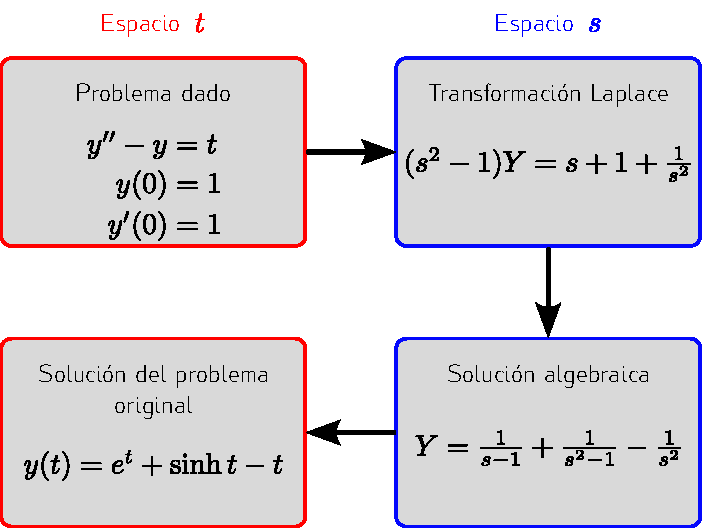
\includegraphics[scale=0.55]{figs/fig-02.pdf}
		\end{center}
	\end{columns}
\end{frame}

\begin{frame}{Teoremas de corrimiento}
	\begin{columns}[t]
		\cx
		\begin{theorem}[Corrimiento $s$]
			Si $f(t)$ tiene transformada $F(s)$ ($s > k$ para algún $k$), entonces:
			\[ \mathscr{L}[e^{at} f(t)] = F(s -a) \]
			o, antitransformando miembro a miembro:
			\[ e^{at} f(t) = \mathscr{L}^{-1} [F(s -a)] \]
			donde $s - a > k$.
		\end{theorem}

		\cx
		\begin{theorem}[Corrimiento $t$]
			Si $f(t)$ tiene transformada $F(s)$, entonces la \textbf{función desplazada}
			\[ \tilde{f}(t) = f(t - a) H(t - a) =
				\begin{cases}
					0        & \text{ si } t < a \\
					f(t - a) & \text{ si } t > a
				\end{cases}
			\]
			tiene transformada $e^{-a s} F(s)$, es decir:
			\[ \mathscr{L}[f(t - a) H(t - a)] = e^{-a s} F(s) \]
			o, tomando antitransformadas:
			\[ f(t -a) H(t-a) = \mathscr{L}^{-1}[e^{- a s} F(s)] \]
		\end{theorem}
	\end{columns}
\end{frame}

\begin{frame}{Convolución}
	\begin{columns}[t]
		\cx
		La convolución de dos funciones $f$ y $g$ es un caso particular de \textbf{transformación integral}, y se define como:
		\[ c(t) = (f * g)(t) = \int_{-\infty}^{\infty} f(\tau) g(t - \tau) \, d\tau \]
		o equivalentemente
		\[ c(t) = (f * g)(t) = \int_{-\infty}^{\infty} f(t - \tau) g(\tau) \, d\tau \]

		\cx
		\begin{theorem}[Convolución]
			Si dos funciones $f$ y $g$ satisfacen la restricción de crecimiento exponencial, de modo que sus transformadas $F$ y $G$ existen, el producto $C = FG$ es la transformada de $(f * g)$.
		\end{theorem}
	\end{columns}
\end{frame}

\section*{Bibliografía}
\begin{frame}{Lecturas recomendadas}
	\begin{itemize}
		\item \fullcite{kreyszig2011}. Capítulo 6.
		\item \fullcite{oneil2012es}. Capítulo 1.
		\item \fullcite{stroud2020}. Programas 2, 3 y 4.
	\end{itemize}
\end{frame}

\end{document}

